\section{Produktrealisering \label{sec:produktrealisering}}

\subsection{KEP-branding \label{sec:kep-branding}}
KEP er en imaginær privat virksomhed, der står for at udvikle og distribuere applikationen samt hoste dataene, denne nedhenter. >>KEP<< er et akronym, der står for >>Krisemanual- og ernærningsberegningsprogram<<. Akronymet eksistens begrundes i, at det fulde navn er for langt til at være memorabelt og genkendeligt.

KEP har ligedan et logo og en farvepalette, (læs mere om farvepaletten i sektionen om design \ref{sec:design}). Logoet er simpelt og består af akronymet KEP. Logoet er lavet med skrifttypen Bebas Neue, hvorefter denne er blevet modificeret, så den minder mere om DRs gamle logo: 
\begin{figure}[H]
    \centering
    \fbox{
\includegraphics[width=0.5\textwidth]{assets/section_8/DR_logo_(1964-1996).png}}
    \caption{Viser logoet for DR (1964-1996), som er blevet brugt som inspiration til KEPs logo}
\end{figure}

Der tages udgangspunkt i DRs logo, da det er æstetisk samt signalerer stabilitet og troværdighed.

Selve logoet er blevet lavet i Inkscape\footnote{>>Inkscape<< er et gratis vektorgrafikprogram.}, via vektorgrafik, så det kan genanvendes på forskellige måder, uden at miste kvaliteten samt skaleres. 

Hertil er trinvisforbedring anvendt til at skabe logoet. Forneden er nogle af iterationerne, som logoet har gennempet:
\begin{figure}[H]
    \centering
    \fbox{\includegraphics[width=0.5\textwidth]{assets/section_8/iteration1.png}}
    \caption{Viser første udkast til logoet.}
\end{figure}

\begin{figure}[H]
    \centering
    \fbox{
\includegraphics[width=0.5\textwidth]{assets/section_8/2iteration.png}}
    \caption{Viser andet udkast til logoet.}
\end{figure}

Herefter det endelige logo:
\begin{figure}[H]
    \centering
    \fbox{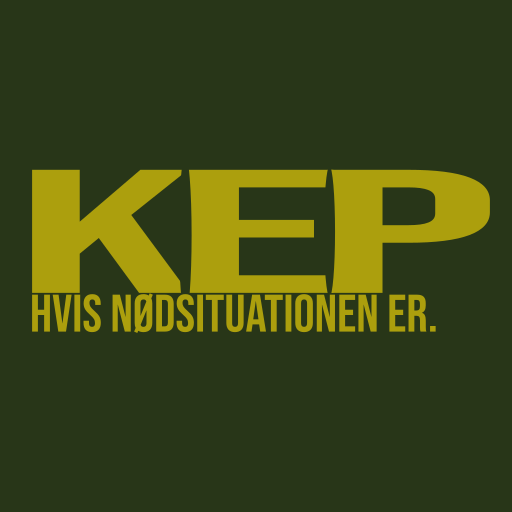
\includegraphics[width=0.5\textwidth]{assets/section_8/icon.png}}
    \caption{Viser det endelige logo.}
\end{figure}

% Her skrives om branding af virksomheden, KEP.
% Henvis til dette kapitel i kapitlet med HV-modellen, hvor "KEP-størrelsen" benævnes og derved først introduceres.
\subsection{Profiteringsmodel \label{sec:profiteringsmodel}}
% Heri beskrives, hvordan appen gøres profitabel.
% Forsikringsbaseret model, der tillader månedlig abonnoment, der oplåser den nyeste version af appen, hvilket tillader løbende udvikling mhp. krisesikre brugeren mod diverse hypotetiske situationer. 

For at gøre appen profitabel, vil denne koste et gebyr for at anvende. Grundet kriteriet om at appen skal være tilgængelig uden internetforbindelse (jf. kapitlet om produktprincip \ref{sec:produktprincip}), vil det være umuligt at gøre således, at appejerskab kontrolleres, såfremt der betales regulært, når denne startes. Herfor er er det ikke muligt at gøre tjenesten abonnoment-baseret.

Derfor er det valgt, at appen koster et engangsgebyr, hvorefter yderligere DLC-pakker\footnote{>>DLC<< står for >>Downloadable Content<<.} vil kunne tilkøbes, hvilket vil give mulighed for løbende udvikling mhp. at krisesikre brugeren mod diverse hypotetiske situationer. I takt med, at det vurderes, at efterspørglen efter appen stiger, vil priserne for disse pakker og grundkøbet hæves løbende og ligedan sænkes, hvis efterspørgslen vurderes lavere.

For at sikre KEPs interesser jf. overstående, da er det essentielt, at koden ikke viderdeles af ikke-autoriserede personer eller organisationer. Således vil der i appens TOU\footnote{>>TOU<< står for >>Terms of Use<< og beskriver hvilke vilkår og regler, en bruger skal overholde for at kunne benytte sig af appen} blive beskrevet, hvordan brugeren ikke må vidergive appens kode, ellers vil de kunne retforfølges for erstating som måtte følge heraf. Ligedan vil appens ideer og struktur blive patenteret, hvorfor andre virksomheder ikke vil kunne udvikle en applikation magen til. Desuden vil diverse brand- og logokomponenter blive varemærket, således at de ikke bliver associeret med andre virksomheder uden KEPs tilladelse, altså er brandopfattelsen indenfor KEPs kontrolsfære, så det kan sikres, at KEP opfattes troværdigt. 

\subsubsection{Etik og ansvar \label{sec:etik-og-ansvar}}
Da appen vil være dyr, må det forventes, at KEP er ansvarlig for at appen har korrekt og brugbart indhold, altså betaler man også for dette som bruger. Ligedan i perioden, hvor appen er gratis, vil KEP ikke være ansvarlig for eventuelle fejl eller mangler i appen. For at sikre indhold af højest mulig kvalitet, vil KEP samarbejde med eksperter og organisationer om at udarbejde dette.
\newpage 
\subsection{Appmarkedsdistribution}
% Heri henvises til kapitlet om Expo, hvori forskellen på Expo Go, som udviklingsværkøj, og appmarkedsdistributionen, som er hvor appen kan downloades til end-consumption.
% om shipping af ikoner.
De to primært anvendt styrestystemer på tablets er iOS\footnote{iOS er Apples styresystem til deres mobile enheder.} og Android\footnote{Android er et linuxbaseret styresystem, som udvikles af Open Handset Alliance, der består af 84 forskellige virksomheder, hvor Google har hovedteten.\cite{Android-wiki}}. 
I Danmark, er har IOS en markedsandel på 65,95\%, hvor Android har en markedsandel på 33,62\%\cite{markedsandelkilde}. Herfor giver det også god mening, at appen er udviklet til at køre på begge dele.

\subsubsection{Apple App Store}
På IOS, er den meste almindelige package manager\footnote{>>package manager<< er en software, der adminisrerer softwarepakker, således at eventuelle softwareafhængigheder installeres. Desuden opdaterer den pakker og kan slette nuværende.} App Store. Dette har længe været den eneste måde at nedhente applikationer på, da det er Apples egen platform, dog på grund af et EU's Digital Markets Act, skal Apple gøre således, at brugere i EU kan tilgå andre pakke-forvaltere.\cite{appleDMA} Således vil KEP også gøre, således at brugere i EU, kan downloade appen direkte fra KEP, uden mellemmand, dog vil den stadig være tilgængelig på App Store og andre pakke-forvaltere på iOS, hvis disse eller bliver udbredt.

\subsubsection{Google Play Store}
På Android, er den meste almindelige package manager Google Play Store. Dog findes der også andre pakke-forvaltere, som f.eks. F-Droid\footnote{>>F-Droid<< er ligesom Google Play Store, en pakke-forvalter til Android, som er open source og gratis.\cite{F-Droid-wiki}}. F-droid har kun applikationer, som er open source\footnote{Indenfor programmering, differentierer man imellem proprietær kode, som kun kan tilgås af ejeren || udvikleren, og open source kode, som kan tilgås og bidrages til af alle.} og gratis, hvilket ikke harmonerer med KEPs profiteringsmodel og kodestruktur \ref{sec:kodestruktur}, som kommer til at være proprietær, hvorfor denne vil ikke være tilgængelig her. 

\subsubsection{Egendistribution - apk}


\subsection{Viderdownload-prompt}.
% Heri henvises til den typiske model i spil, hvor maps, textures, kan downloads, hvis man vil tilgå dem.